

%====================
\section{One Dimensional Contact}
%====================

\subsection{Concepts}
\subsubsection{Gap and Penetration}
Consider two bodies $\cA$ and $\cB$ in moving in inertial reference from $\cF$ with origin
$O$ and basis vector $\vefa$, as shown in Fig.~\ref{fig:1D_contact}.
Let point $P$ be located on the right-hand-side of body $\cA$, denoting the first contact surface
$\partial \cA$.
Let point $Q$ be located on the left-hand-side of body $\cB$, denoting the second contact surface
$\partial \cB$.  Let the contact boundaries be denoted as $\Gamma_c = \partial \cA \union \partial \vB$. 
Let the time evolution from $t=0$ (initial) to $t=T$ (final) be denoted as $\interval = [0, T] \subset \realplus$.
At the initial time $t=0$, these two points are located by $X^{OP}$ and $X^{OQ}$, respectively.
%\begin{figure}[htb]
%  \psfrag{A}{$\cA$}
%  \psfrag{a}{$\vefa$}
%  \psfrag{B}{$\cB$}  
%  \psfrag{F}{$\cF$}
%  \psfrag{G}{$g_0$}  
%  \psfrag{g}{$g$}    
%  \psfrag{O}{$O$}
%  \psfrag{P}{$P$}
%  \psfrag{p}{$p$}  
%  \psfrag{Q}{$Q$}
%  \psfrag{R}{$t=t_0 = 0$}
%  \psfrag{S}{$t=t_1 > 0$}
%  \psfrag{T}{$t=t_2 = 3 t_1$}    
%  \psfrag{X}{$X^{OP}$}
%  \psfrag{x}{$\varphi^{OP}(t_1)$}
%  \psfrag{u}{$\varphi^{OP}(t_2)$}
%  \psfrag{Y}{$X^{OQ}$}    
%  \psfrag{y}{$\varphi^{OQ}(t_1)$}    
%  \psfrag{v}{$\varphi^{OQ}(t_2)$}      
%  \begin{center}
%   %\includegraphics[width=4.5in]{../AR/ARfinal.eps}
%   %\includegraphics[width=4.5in]{../AR/AR_diagram_CBH.eps}
%   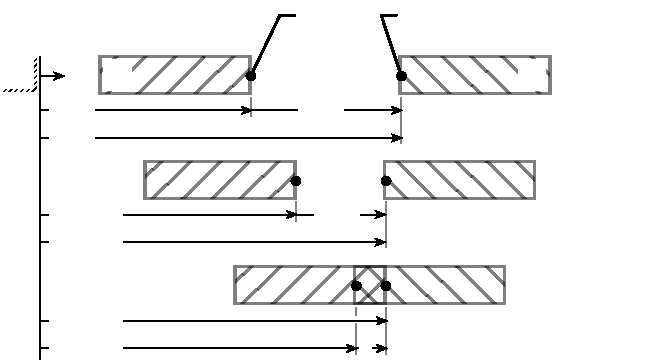
\includegraphics[width=0.9\textwidth]{fig/1D_contact}
%   %\includegraphics[width=3.5in]{../../AR/referenceFramesTwo.eps}
% \end{center}
% \caption{Caption to come.}
% \label{fig:1D_contact}
%\end{figure}

\begin{figure}[htb]
  \begin{center}
  %\begin{overpic}[width=\textwidth, grid, tics=10]{fig/1D_contact}
  \begin{overpic}[width=\textwidth]{fig/1D_contact}
  \put(17, 43.5){$\cA$}
  \put(81, 43.5){$\cB$}
  %
  \put(11, 43){$\vefa$}
  \put( 2, 43){$\cF$}
  %
  \put(48.5, 38){$g_0$}  
  \put(51.5, 22){$g$}    
  \put(56,  1){$p$}  
  %
  \put( 8, 47){$O$} 
  \put(46.5, 52.5){$P$}
  \put(62.5, 52.5){$Q$}
  %
  \put(88, 44){$t=t_0 = 0$}
  \put(88, 28){$t=t_1 > 0$}
  \put(88, 12){$t=t_2 = 3 t_1$}    
  %
  \put( 8.5, 38){$X^{OP}$}
  \put( 8.5, 33.5){$X^{OQ}$}    
  %
  \put( 8.5, 22){$\varphi^{OP}(t_1)$}
  \put( 8.5, 17.5){$\varphi^{OQ}(t_1)$}    
  %
  \put( 8.5,  5.5){$\varphi^{OP}(t_2)$}
  \put( 8.5,  1){$\varphi^{OQ}(t_2)$}      
 \end{overpic}
 \end{center}
 \caption{Caption to come.}
 \label{fig:1D_contact}
\end{figure}

At $t=0$, the initial gap $g_0 : [\Gamma_c \times 0] \mapsto \realplus$ 
between the two points $P$ and $Q$ is given by
\be
 g(t=0) = g_0 = X^{OQ} - X^{OP} \defe X^{PQ}, \hspace{1cm} g_0 > 0.
\ee
In general, the gap $g : [\Gamma_c \times \interval] \mapsto \real$ between the points is given by
\be
 g(\vvarphi(\vX), t) = \varphi^{OQ}_t - \varphi^{OP}_t = (X^{OQ} + u^Q_t) - (X^{OP} + u^P_t) = g_0 + u^Q_t - u^P_t,
\ee
where $u_t$ is a displacement, 
$\varphi_t$ is a current configuration, 
$\vu = \langle u^P_t, u^Q_t \rangle^T$, and
$\vvarphi = \langle \varphi^{OP}_t, \varphi^{OQ}_t \rangle^T$.
For arbitrary displacements $u^P_t$ and $u^Q_t$, the gap can be either positive, negative, or zero.
For example, at $t=t_2$, the gap is negative.  It is useful, as will seen in subsequent discussions on the penalty formulation ({\em see} ??), 
to define penetration $p$ as the negative of the gap.  
The penetration $p : [\Gamma_c \times \interval] \mapsto \real$ is defined as
\be
  p(\vu, t) \defe -g(\vu, t) = - \varphi^{OQ}_t + \varphi^{OP}_t = - (X^{OQ} + u^Q_t) + (X^{OP} + u^P_t) = - g_0 - u^Q_t + u^P_t.
\ee
Note that
\be
 p(t=0) = p_0 = - g_0, \hspace{1cm} p_0 < 0.
\ee

\subsubsection{Non-Penetration}
The penetration of body $\cA$ and body $\cB$, shown (for example) at $t=t_2$ in Fig.~\ref{fig:1D_contact}, is prevented
by constraining the gap $g$ (or, equivalently, the penetration $p$) as follows:
\begin{align}
 g &\geq 0, \\
 p &\leq 0.
\end{align}

Theses two inequality conditions are {\bf unilateral constraints} on the motion $\vvarphi$.  To illustrate
the unilateral constraint concept in a concrete sense, consider $\cB$ in Fig.~\ref{fig:1D_contact} to be 
stationary for all time.  Thus $u^Q_t = 0$, and we can abbreviate the displacement of body $\cA$ as 
$u^P_t = u$.  The gap and penetration functions are then
\begin{align}
 g(u) & = g_0 - u, \\
 p(u) & = -g(u) = u - g_0 = u + p_0.
\end{align}
Assume, for concreteness $g_0 = 1$~m.  The gap and penetration functions are then shown in
Fig.~\ref{fig:1D_gap_penetration}.

\begin{figure}[htb]
  \psfrag{a}{$(0, g_0)$}
  \psfrag{b}{$(g_0, 1)$}
  \psfrag{c}{$(-p_0, 0)$}
  \psfrag{d}{$(1, p_0)$}
  \psfrag{e}{$g(u) \geq 0$}
  \psfrag{f}{inadmissible}
  \psfrag{g}{inadmissible}
  \psfrag{h}{$p \leq 0$}
  \psfrag{s}{$\subset u \implies$ $g \geq 0$}
  \psfrag{t}{$\subset u \implies$ $p \leq 0$}    
  \begin{center}
   %\includegraphics[width=4.5in]{../AR/ARfinal.eps}
   %\includegraphics[width=4.5in]{../AR/AR_diagram_CBH.eps}
   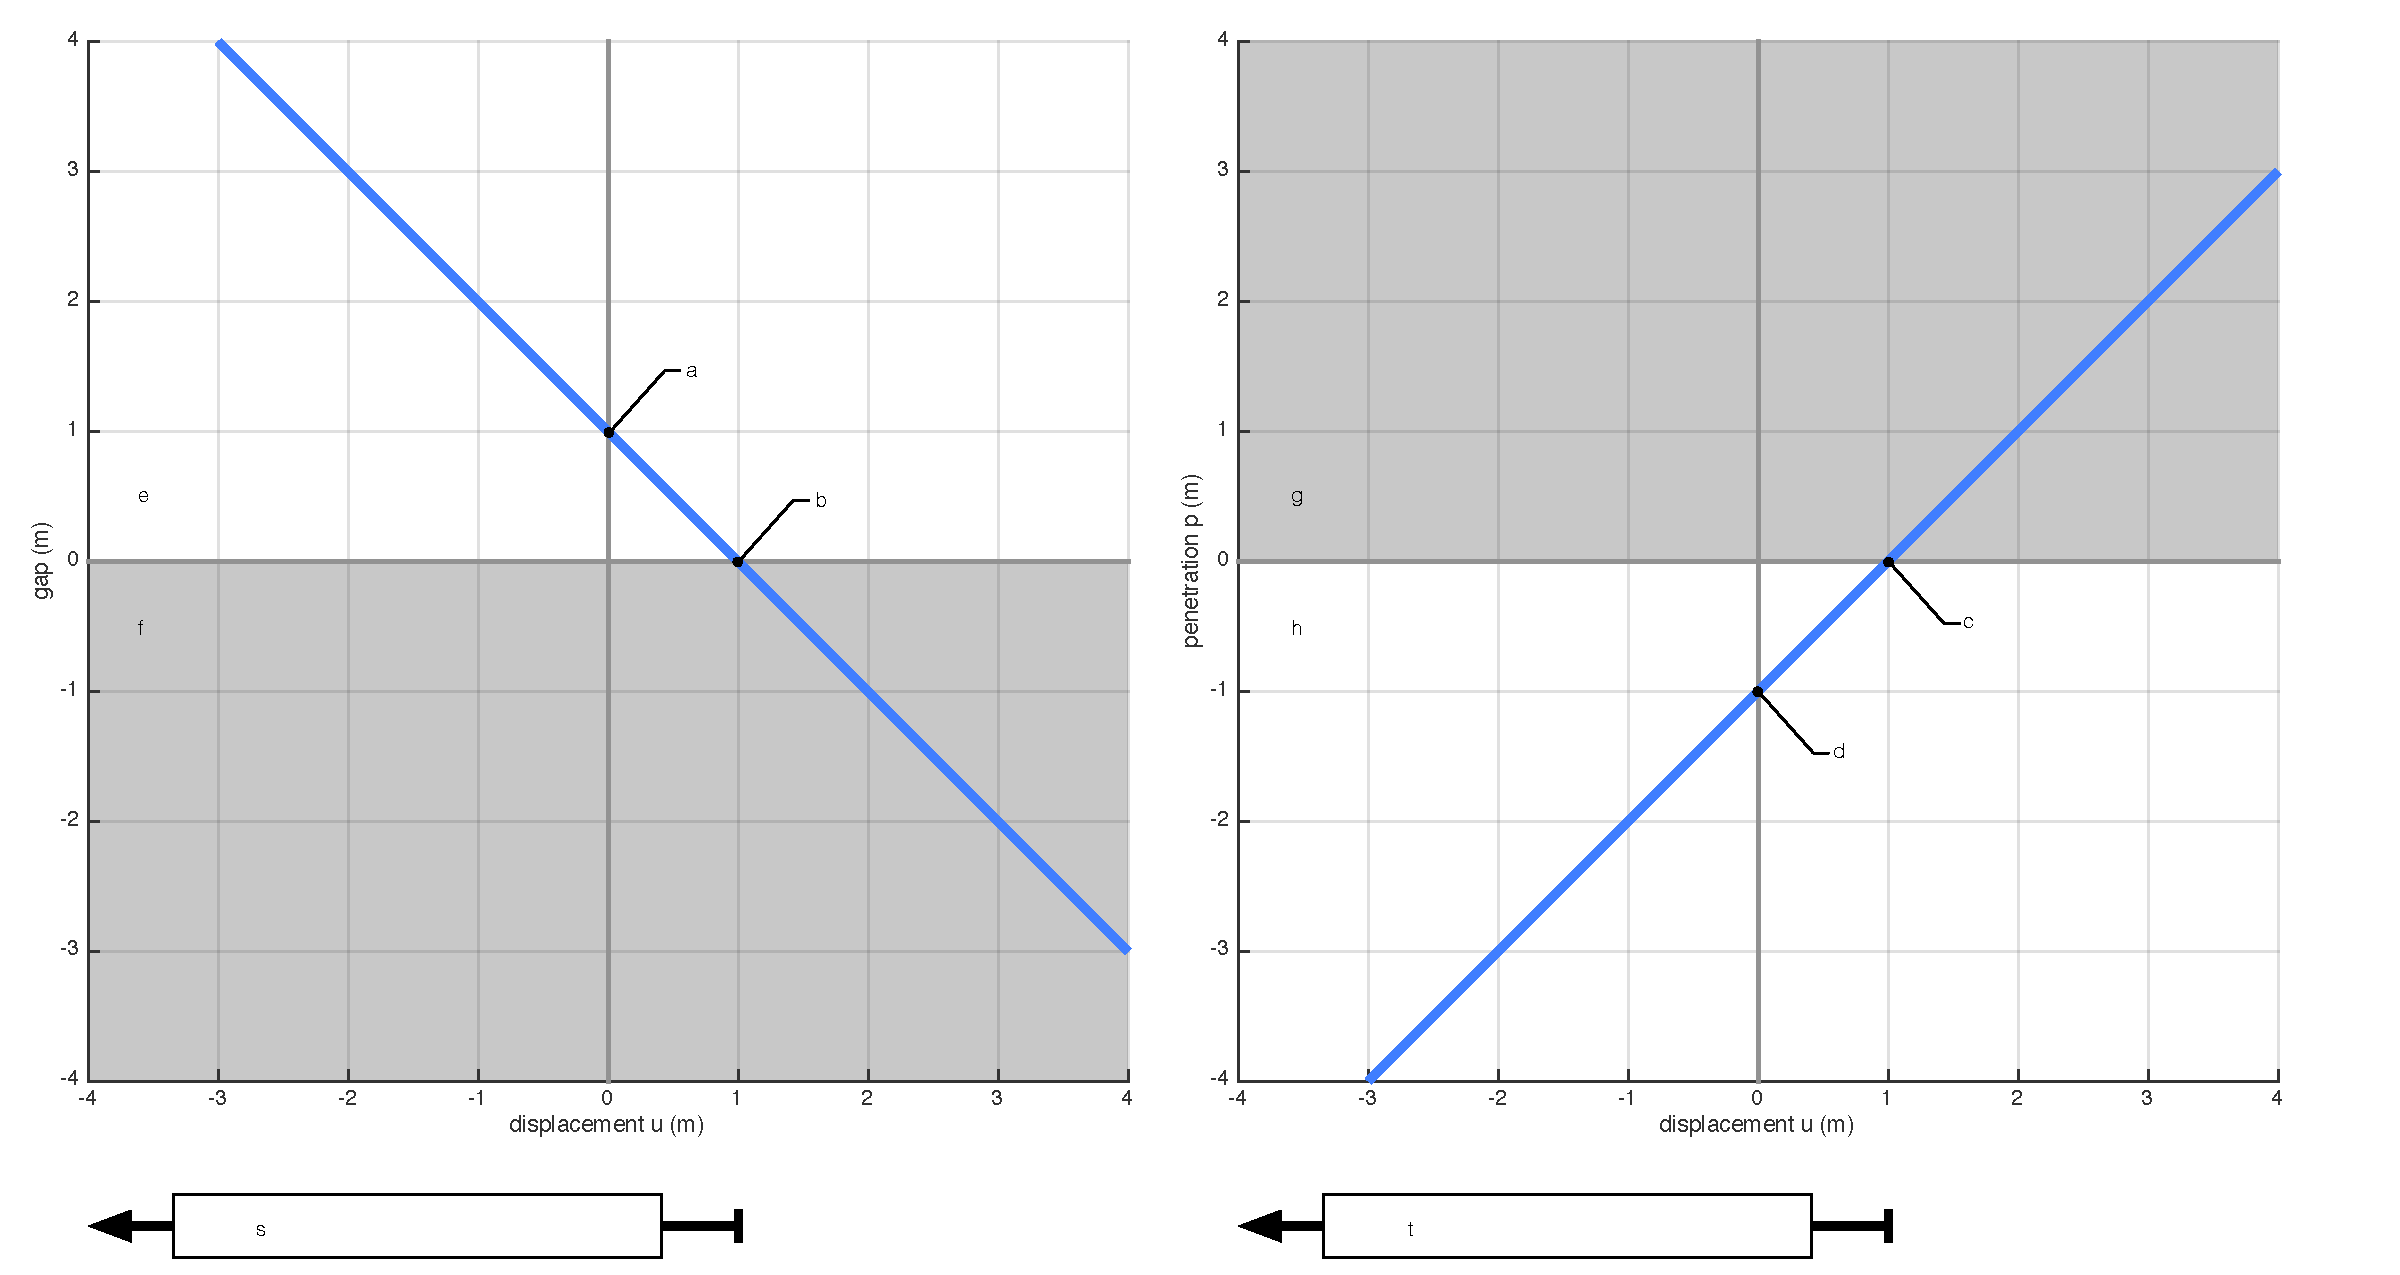
\includegraphics[width=\textwidth]{fig/1D_gap_penetration}
   %\includegraphics[width=3.5in]{../../AR/referenceFramesTwo.eps}
 \end{center}
 \caption{Caption to come.}
 \label{fig:1D_gap_penetration}
\end{figure}


\subsection{Example with Spring and Weight}
We start by considering a spring mass system, with spring constant $k$, mass $m$, gravitational field
$-g \; \vefb$, with the spring initially unstretched at $t=t_0 = 0$, as shown in Fig.~\ref{fig:1D_spring_mass}.  While this example does not yet have contact, it sets the context of energy minimization as method used to find static equilibrium.  

\begin{figure}[htb]
  \psfrag{0}{$0$} \psfrag{1}{$1$} 
  \psfrag{a}{$\vefa$}
  \psfrag{b}{$\vefb$}
  \psfrag{k}{$k$}    
  \psfrag{m}{$m g$} 
  \psfrag{n}{$-1$}       
  \psfrag{O}{$O$}
  \psfrag{R}{$t=t_0 = 0$}
  \psfrag{S}{$t=t_1 > 0$}
  \psfrag{X}{$X^{OP}$}
  \begin{center}
   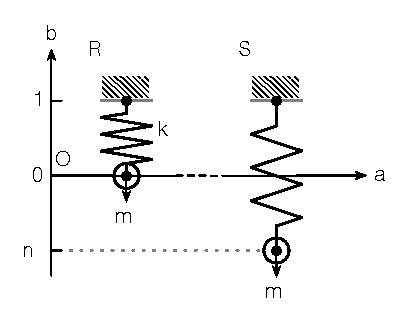
\includegraphics[width=0.5\textwidth]{fig/1D_spring_mass}
 \end{center}
 \caption{Caption to come.}
 \label{fig:1D_spring_mass}
\end{figure}

For concreteness, let $k=2$~N/m, $m=0.2$~kg, and $g=10$~m/s${^2}$, (for simplicity, rounded up from $9.81$~m/s${^2}$).  Let displacement $u$ of the mass, initially at $0$, be measured in the $\vefb$ axis.  
The internal energy (IE) of the spring as a function of $u$ is given by $\Pi_{k}(u) = \half k u^2$.
The potential energy (PE) of the mass as a function of $u$ is given by $\Pi_{m}(u) = m g u$.
Minimization of the potential energy gives
\begin{align}
 \delta \Pi = & \; \delta \left(\Pi_{k}(u) + \Pi_{m}(u) \right) = 
 \delta \left(\half k u^2 + m g u \right) = \left( k u + m g \right) \delta u \setequal 0, \\
 \implies u = & \; \frac{-m g}{k} = \frac{-0.2 \cdot 10}{2} = -1.
\end{align}

\begin{figure}[htb]
  \begin{center}
   %\includegraphics[width=4.5in]{../AR/ARfinal.eps}
   %\includegraphics[width=4.5in]{../AR/AR_diagram_CBH.eps}
   \includegraphics[width=0.8\textwidth]{fig/1D_spring_mass_plot_trim.eps}
   %\includegraphics[width=3.5in]{../../AR/referenceFramesTwo.eps}
 \end{center}
 \caption{Caption to come.}
 \label{fig:1D_spring_mass_plot}
\end{figure}

Fig.~\ref{fig:1D_spring_mass_plot} shows the spring internal energy, $\Pi_{k}(u)$, in dashed blue, which shows a minimum 
at $u=0$, and a symmetric, parabolic response for nonzero displacements, as expected.
The potential energy due to the mass, $\Pi_{m}(u)$, is shown in dot-dash green, which shows a linear relationship in $u$ with intercept $0$ and slope $m g = 0.2 \cdot 10 = 2$~N.

The addition of the two aforementioned potentials, $\Pi(u) = \Pi_{k}(u) + \Pi_{m}(u)$, is shown in solid red.
The system potential, $\Pi(u)$, has a minimum at $u=-1$~m, as expected.
Next, we used this concept of minimizing potential energy in the context of contact.

\subsection{Example with Spring and Rigid Wall}
Consider a spring, shown in Fig.~\ref{fig:1D_spring_wall}, with elastic constant $k = 2$~N/m, undeformed length $L_0 = 2$~m subjected to a prescribed displacement in the amount of $\bar{u} = 2$~m on the left-hand-side.\footnote{This example follows Laursen TA (2013), {\em Computational contact and impact mechanics: fundamentals of modeling interfacial phenomena in nonlinear finite element analysis.} Springer Science \& Business Media, page 87.}
A rigid wall is $g_0 = X^{PQ} = 1$~m from the right-hand-side of the spring at $t=0$.
At $t=t_1$, the spring has undergone its prescribed displacement and penetrates the wall by amount $p$.  
In this configuration, internal energy $\Pi$ for the spring for the as a function of $u = u^P$ is given by
\be
 \Pi(u) = \frac{1}{2} \; k \; \delta^2 = \frac{1}{2} \; 2 \; (u - \bar{u})^2 = (u - 2)^2 \; (\mbox{Nm}).
\ee

\begin{figure}[htb]
  \psfrag{0}{$0$} \psfrag{1}{$1$} \psfrag{2}{$2$} \psfrag{3}{$3$} \psfrag{4}{$4$}
  \psfrag{A}{$\cA$}
  \psfrag{a}{$\vefa$}
  \psfrag{B}{$\cB$}  
  \psfrag{c}{$\bar{u}$}
  \psfrag{d}{$\bar{u}=2$}
  \psfrag{F}{$\cF$}
  \psfrag{G}{$g_0$}  
  \psfrag{g}{$g$}    
  \psfrag{k}{$k$}      
  \psfrag{O}{$O$}
  \psfrag{P}{$P$}
  \psfrag{p}{$p$}  
  \psfrag{Q}{$Q$}
  \psfrag{R}{$t=t_0 = 0$}
  \psfrag{S}{$t=t_1 > 0$}
  \psfrag{T}{$t=t_2 > t_1$}    
  \psfrag{X}{$X^{OP}$}
  \psfrag{x}{$\varphi^{OP}(t_1)$}
  \psfrag{u}{$\varphi^{OP}(t_2)$}
  \psfrag{Y}{$X^{OQ}$}    
  \psfrag{y}{$\varphi^{OQ}(t_1)$}    
  \psfrag{v}{$\varphi^{OQ}(t_2)$}      
  \begin{center}
   %\includegraphics[width=4.5in]{../AR/ARfinal.eps}
   %\includegraphics[width=4.5in]{../AR/AR_diagram_CBH.eps}
   \includegraphics[width=0.5\textwidth]{fig/1D_spring_wall.eps}
   %\includegraphics[width=3.5in]{../../AR/referenceFramesTwo.eps}
 \end{center}
 \caption{Caption to come.}
 \label{fig:1D_spring_wall}
\end{figure}





\subsubsection{Principle of Minimum Potential Energy}
\subsubsection{Principle of Minimum Potential Energy with Lagrange Multiplier Enforcement}


\begin{figure}[htb]
  \psfrag{t}{$\subset u \implies$ $p \leq 0$}    
  \begin{center}
   %\includegraphics[width=4.5in]{../AR/ARfinal.eps}
   %\includegraphics[width=4.5in]{../AR/AR_diagram_CBH.eps}
   \includegraphics[width=0.8\textwidth]{fig/1D_spring_with_wall_trim_soln.eps}
   %\includegraphics[width=3.5in]{../../AR/referenceFramesTwo.eps}
 \end{center}
 \caption{Caption to come.}
 \label{fig:1D_spring_with_wall_soln}
\end{figure}

\clearpage

\begin{figure}[htb]
  \psfrag{a}{$\lambda = 0$}
  \psfrag{b}{$\lambda = \half$}  
  \psfrag{c}{$\lambda = 1$}
  \psfrag{d}{$\lambda = 2$}
  \psfrag{e}{$\lambda = 3$}
  \psfrag{f}{$\lambda = 4$}  
  \psfrag{g}{$\lambda = 5$}    
  \psfrag{h}{$\lambda = 6$}      
  \psfrag{t}{$\subset u \implies$ $p \leq 0$}    
  \begin{center}
   %\includegraphics[width=4.5in]{../AR/ARfinal.eps}
   %\includegraphics[width=4.5in]{../AR/AR_diagram_CBH.eps}
   \includegraphics[width=\textwidth]{fig/1D_spring_with_wall_new_trim.eps}
   %\includegraphics[width=3.5in]{../../AR/referenceFramesTwo.eps}
 \end{center}
 \caption{Caption to come.}
 \label{fig:1D_spring_with_wall}
\end{figure}

\begin{align}
 \Pi(u) & = \Pi_k(u) + \Pi_c(u). \\
 & = \half k \left(u - \bar{u}\right)^2 + \lambda p(u). \\
 & = \left(u - \bar{u}\right)^2 + \lambda (u + p_0). \\
 & \mbox{where} \; \bar{u} = 2~\mbox{m}, \; \mbox{and} \; p_0 = -1~\mbox{m}.
\end{align}


\begin{figure}[htb]
  \psfrag{a}{(a)}
  \psfrag{b}{(b)}
  \psfrag{c}{(c)}
  \psfrag{d}{(d)}
  \begin{center}
   \includegraphics[width=\textwidth]{fig/1D_spring_with_wall_iso_trim.eps}
 \end{center}
 \caption{Caption to come.}
 \label{fig:1D_spring_with_wall_iso}
\end{figure}


\subsubsection{Principle of Minimum Potential Energy with Penalty Enforcement}
\subsubsection{Principle of Minimum Potential Energy with Augmented Lagrange Multiplier Enforcement}



%====================
%\pagebreak
%\appendix
%\section{Numerical Details}
%====================


\end{document}







